%************************************************
\chapter{Example Chapter}\label{ch:implementation}
%************************************************

This chapter gives you some examples how to include graphics, create tables, or include code listings.
Examples on how to cite papers from the literature can be found in \autoref{ch:relatedwork}.

\section{Acronyms}

This template makes advantage of the acronyms package to support acronyms. The first occurence of an acronym is replaced by its definition (e.g., \ac{IDE}). All other occurences are replaced by the acronym (\ac{IDE}). The glossaries package also supports plural---\acp{IDE}.

\section{Graphics}

In \autoref{fig:ex}, we give a small example how to insert and reference a figure.

\begin{figure}[htbp]
	\centering
		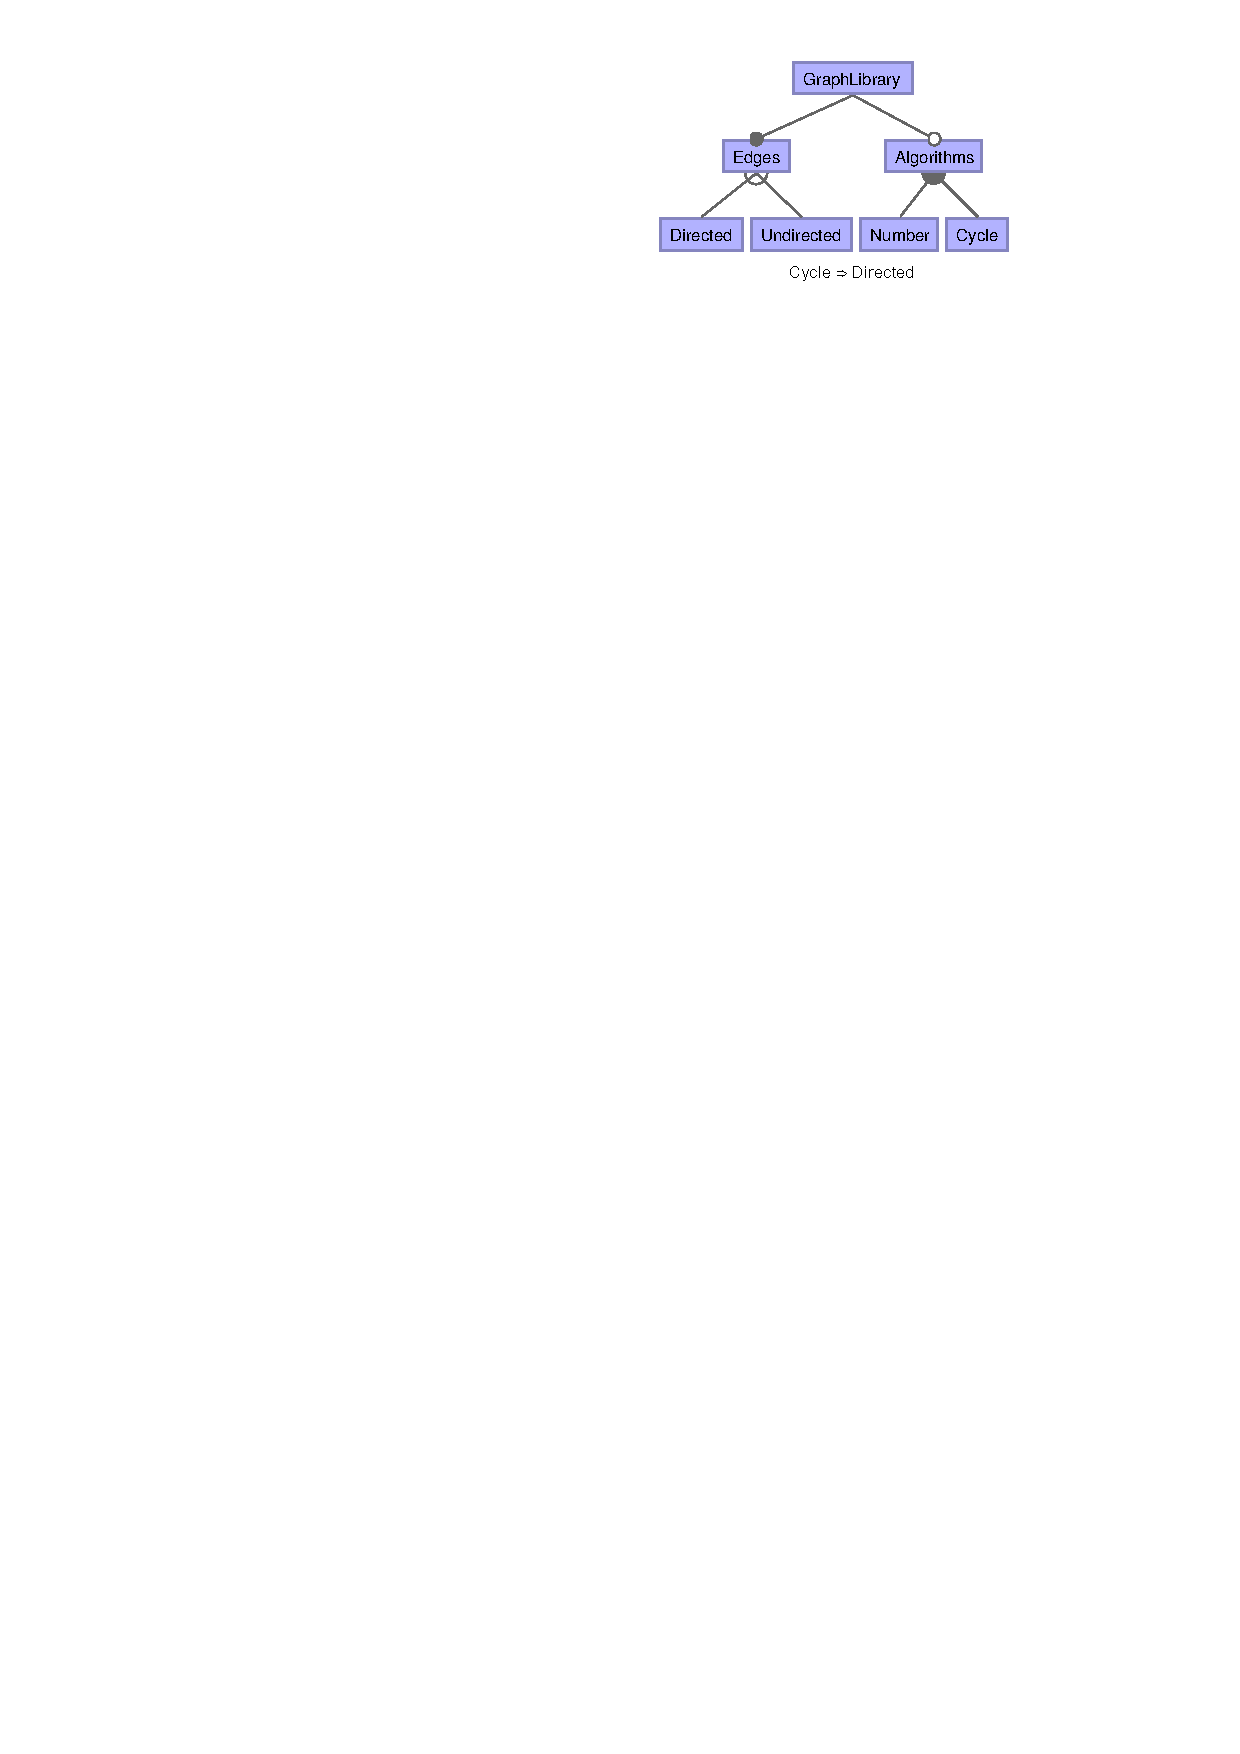
\includegraphics[scale=1.25]{gfx/example}
	\caption{A feature model representing a graph product line}
	\label{fig:ex}
\end{figure}

\section{Tables}

\autoref{tab:ex} shows the result of a simple tabular environment.

\begin{table}[htbp]
        \caption{Mapping a feature model to a propositional formula} 
	\centering
		\begin{tabular}{cc}\toprule
			Group Type & Propositional Formula\\\midrule
			And & $(P \Rightarrow C_{k_1} \wedge\ldots\wedge C_{k_m}) \land (C_1\vee\ldots\vee C_n \Rightarrow P)$\\\addlinespace
			Or & $P = C_1\vee\ldots\vee C_n$\\
			Alternative & $(P = C_1\vee\ldots\vee C_n) \land \mbox{atmost}1(C_1,\ldots,C_n)$\\
			\bottomrule
		\end{tabular}
	\label{tab:ex}
\end{table}

\section{Code Listings}

In \autoref{lst:ex}, we give an example of a source code listing. 

\begin{lstlisting}[language=Java,float=htb,caption={Java source code},label={lst:ex}]
class A extends Object {
	A() { super(); }
}
class B extends Object {
	B() { super(); }
}
class Pair extends Object {
	Object fst;
	Object snd;
	Pair(Object fst, Object snd) {
		super(); this.fst=fst; this.snd=snd;
	}
	Pair setfst(Object newfst) {
		return new Pair(newfst, this.snd);
	}
}
\end{lstlisting}
